\section{Material und Methoden}
\subsection{Laufbandversuch}
\begin{wrapfigure}[18]{r}{5cm}
	\vspace{-40pt}
	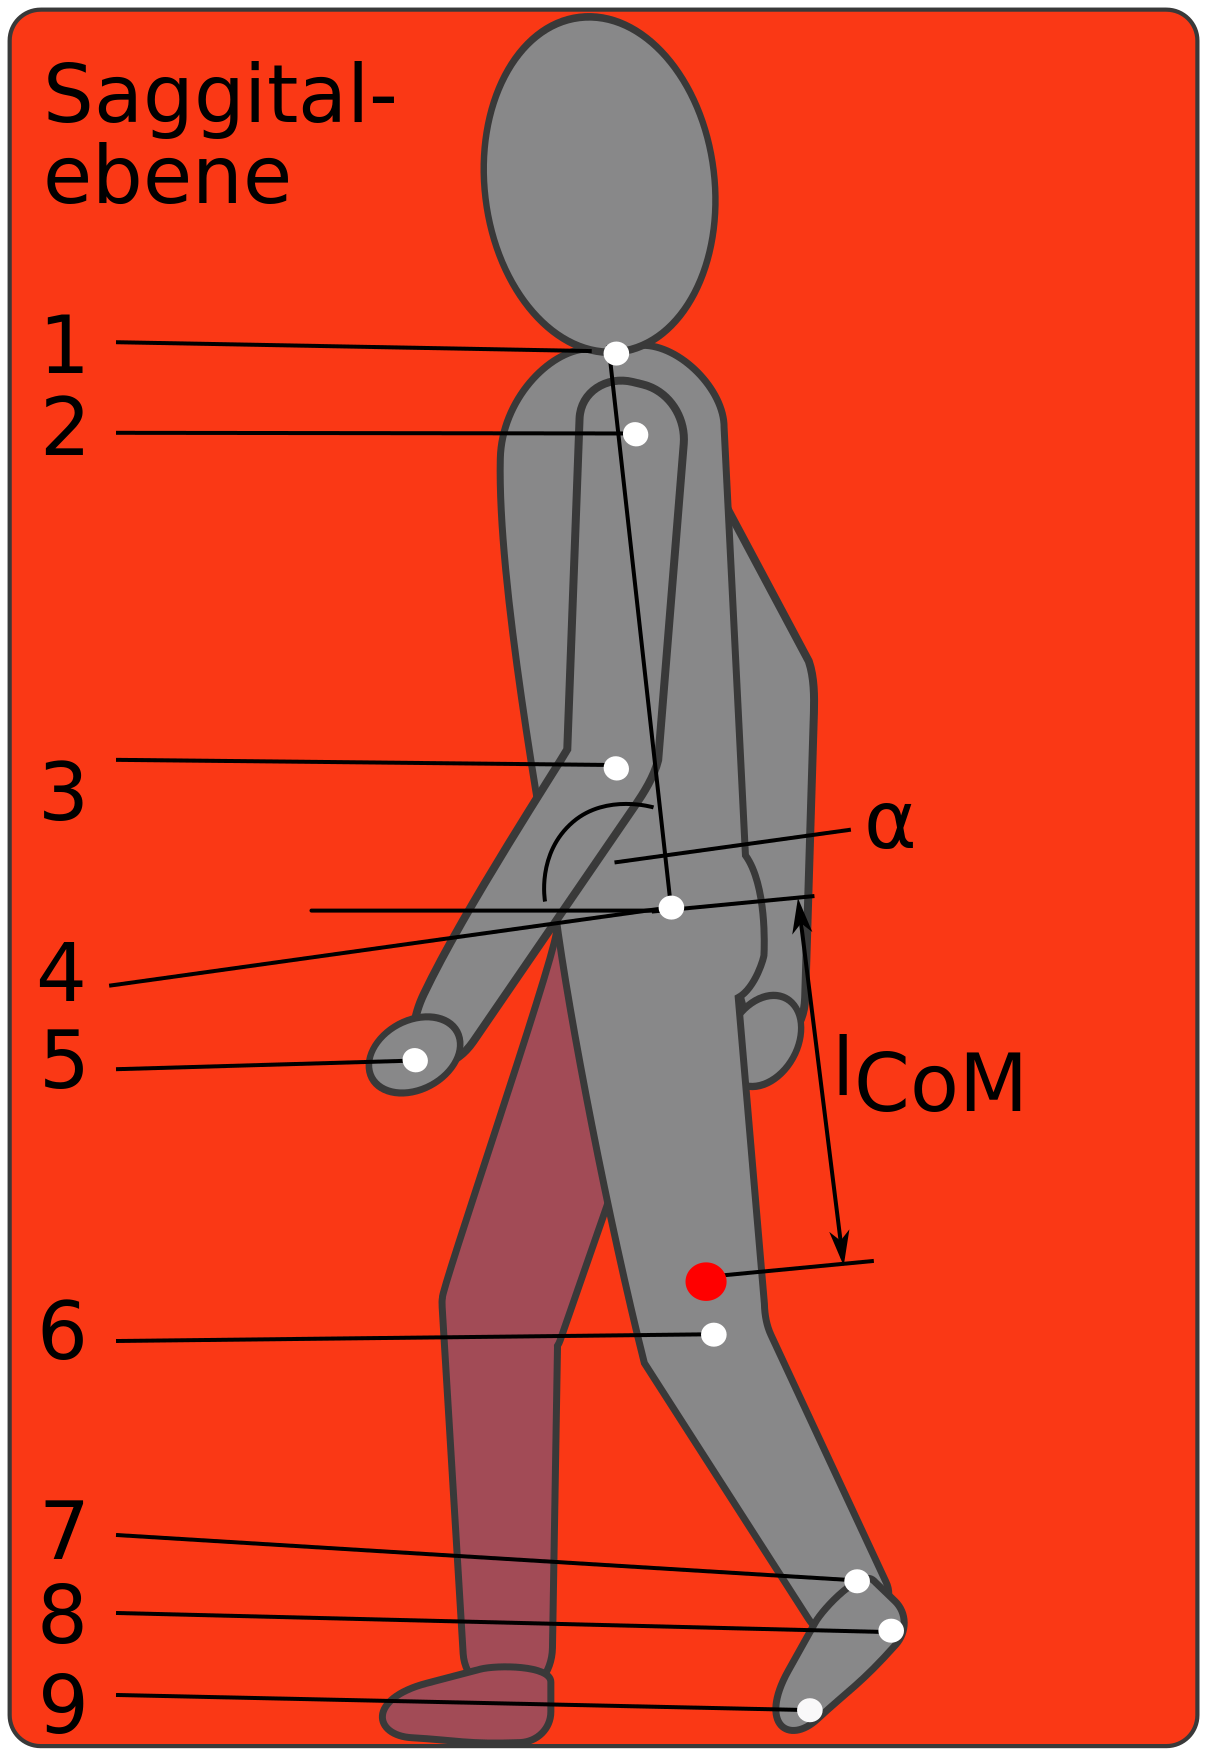
\includegraphics[width=\linewidth]{bilder/Einleitung/Proband_Pendel}
	\vspace{-23pt}
	\caption[Untersuchte Parameter]{Skizze des Probanden in Sagittalebene mit 9 Markern: Nacken~1, Schulter~2, Ellenbogen~3, Hüfte~4, Handgelenk~5, Knie~6, Knöchel~7, Ferse~8 und Ballen~9. Länge des virtuellen Pendels ($l_{CoM}$) von Hüfte zu Massenschwerpunkt (roter Kreis), Oberkörperwinkel ($\alpha$) und Kniewinkel ($\beta$). Pfeil markiert Laufrichtung}
	\label{fig:Proband_Pendel}
\end{wrapfigure}
Der gesunde Proband ist 25 Jahre alt, 75~kg schwer und 1,82~m groß. Er läuft auf Socken und neun Gelenke werden mit reflektierenden Markern versehen (s.~Abb.~\ref{fig:Proband_Pendel}). Der Aufbau (s.~Abb.~\ref{fig:setup_combo}~A) besteht aus einem mercury 4.0 Laufband (h/p/cosmos sports \& medical GmbH, Nussdorf-Traunstein, Deutschland), einer Samsung VP-HMX20C Videokamera (Samsung AG, Seoul, Südkorea) auf einem Manfrotto 496RC2 Stativ (Manfrotto, Cassola, Italien) und zwei weißen 500W GT3E Baustrahlern (Hornbach, Bornheim, Deutschland). Die Kamera steht zentriert vor dem Probanden und die Bildebene ist pa-rallel zur Sagittalebene ausgerichtet. Zur Skalierung dienen zwei Markierungen am Laufband mit 1~m Abstand.\\
Ausgehend von 1~km/h werden in 1~km/h-Schritten sieben Geschwindigkeiten untersucht. Das Gehen wird subjektiv von 1 (angenehm) bis 10 (unangenehm) bewertet. Je zwei Gangzyklen werden mit einer Bildrate von 50~Hz, einer Belichtung von 1/1000~s und auf 5~m fixierten Fokus aufgenommen.\\

\subsection{Laufstreckenversuch}
Die Videokamera-Einstellungen und deren Ausrichtung sowie die Beleuchtung des Laufbandversuches werden übernommen. Der Proband läuft in diesem Experiment über eine Laufstrecke von 1~m Breite und 6~m Länge (Eigenbau Hochschule Bremen, Deutschland). Das Kraft-Messsystem besteht aus einem Quarzkristall-3-Komponenten-Dynanometer Typ 9257B (Kistler Gruppe Winterthur, Schweiz), im Folgenden als Waage bezeichnet, einem Mehrkanal-Ladungsverstärker Typ 5070A (Kistler) und einem Computer (s.~Abb.~\ref{fig:setup_combo}~B). Ein Referenzvideo mit einem Stab von 1~m Länge wird zur Skalierung der Bilder aufgenommen. Ausgehend von der unteren linken Bildecke liegt das Waagenzentrum in den Bildern bei x~=~1,35~m und y~=~0,25~m.\\
Die Waagensignale werden mit 100 Hz und 200~N/V aufgezeichnet. Mit DASYLab (Measurement Computing, Norton, USA) werden die Eingangssignale verarbeitet und alle acht Kanäle im ASCII-Format gespeichert. Für eine 4-Punkt-Kalibrierung wird die Waage in alle drei Raumrichtungen mit 0~kg, 1~kg, 3,6~kg und 7,75~kg für je 30~s belastet. Eine Nullmessung wird in den ersten 10~s jeder Kraftmessung durchgeführt, um den genauen Offset abzuziehen. Um unnatürliche Laufmuster zu verhindern, wird die Distanz zur Waage so gewählt, dass diese im ungestörten Gang getroffen wird. Diese Anpassung wird für drei Geschwindigkeiten durchgeführt, welche subjektiv gewählt und als langsam, normal und schnell eingeschätzt werden.
\begin{figure}[h!]
	\centering
	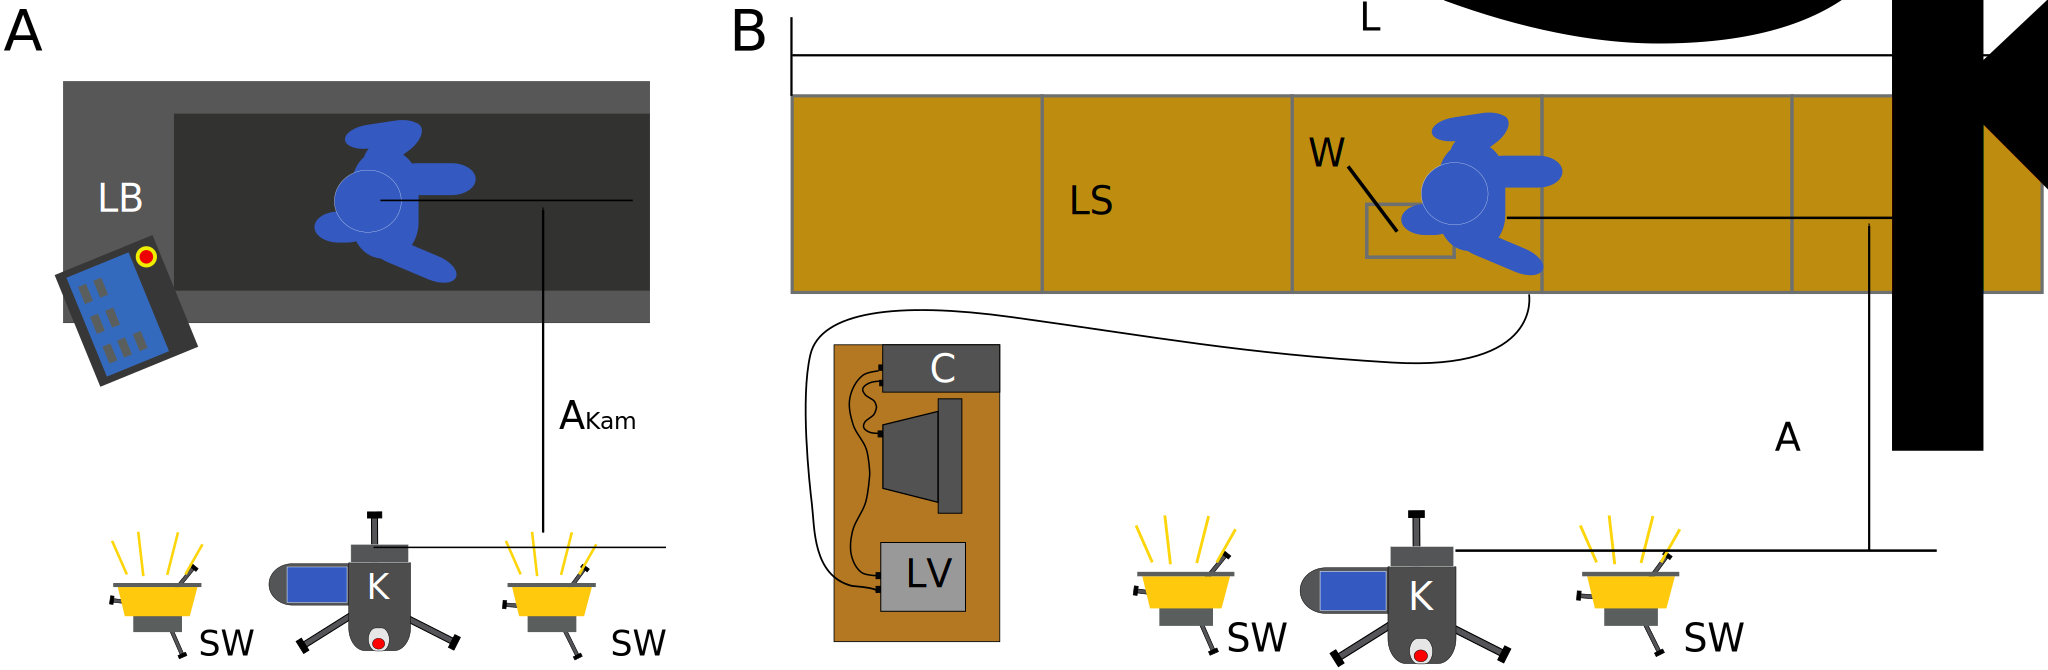
\includegraphics[width=\linewidth]{bilder/mat_met/Setup_combo}
	\caption[Aufbau Laufband- und Laufstreckenversuch]{Aufbau der Experimente mit Laufband~A und Laufstrecke~B. In beiden Versuchen benutzt wurden Kamera K und Scheinwerfer SW. Weitere Komponenten sind Laufband LB, Laufstrecke LS, Computer C, Waage W und Ladungsverstärker. Laufstreckenlänge $L_S~=~6~m$ und Kameraabstand $A_{Kam}~=~5~m$}
	\label{fig:setup_combo}
\end{figure}

\subsection{Datenauswertung}
\paragraph{Rohdatenaufbereitung}
Die Videos werden mit dem Programm ffmpeg 2.1 (LGP License, ffmpeg.org) in Einzelbilder zerlegt und ein Doppelschritt, beginnend mit dem Fersenkontakt, mit wenig bis keinen erkennbaren Störungen pro Geschwindigkeit ausgewählt. In ImageJ (National Institutes of Health, Bethesda, USA) werden mithilfe des Plugins MTrackJ \autocite{meijering2012methods} die X- und Y-Koordinaten aller Gelenke digitalisiert und im .mdf-Format gespeichert. Die Vermessung der Skalierungsbilder ergab eine Länge von 295 px/m und 297 px/m für Laufband- und Laufstreckenversuch. Aufgrund der ca. 0,25~m vor dem Proband befestigten Metermaß auf dem Laufband wurde hier die Körpergröße mit 1,76~m 0,05~m zu ge-ring dargestellt. Mit einer Skalierung von 285 px/m wurde die tatsächliche Körpergröße erreicht, weshalb dieses Verhältnis zur Auswertung genutzt wurde.
\paragraph{Auswertung des Laufbandversuches - mathematisches Pendel}
Die Periodendauer für das mathematische Pendel berechnet sich wie folgt:
\begin{equation}
T = 2 \cdot \pi \sqrt{\frac{l}{g}}
\end{equation}
Für die Berechnung des inversen Pendels wird die Länge l von Ferse bis Hüfte gemessen, die halbe Periodendauer T/2 über die Bildanzahl die Standphase des Beines ermittelt und g gleich der Erdbeschleunigung gesetzt. Für das Schwerkraftpendel ist l gleich der Distanz von Hüfte zum Massenschwerpunkt des Beines und T/2 gleich der Bildanzahl der Schwungphase des Beines. Der Duty-Faktor eines Doppelschrittes errechnet sich aus DF~=~T$_{Stand}$/T$_{Doppelschritt}$.
\subsubsection*{Auswertung in Scilab}
Alle weiteren Auswertungen der Trajektorien und Waagenmessungen werden in Scilab (Scilab Enterprises S.A.S., Orsay Cedex, France) durchgeführt. Für die exakte Implementierung sei auf die beigefügte CD mit dem Quellcode verwiesen.

\paragraph{Numerische Verfahren}
Die grundlegenden Verfahren seien hier für alle Versuche erläutert. Zur Berechnung der Geschwindigkeit eines Punktes wird dessen Ort zeitlich abgeleitet. Die Geschwindigkeit v zum Zeitpunkt t wird mit diskreten Ortswerten $\mathrm{x(t - \Delta{t})}$ und $\mathrm{x(t + \Delta{t})}$ durch Verwendung der Zentraldifferenz berechnet:
\vspace{-5pt}
\begin{equation}
\vec{v}(t) = \frac{\vec{x}(t + \Delta{t}) - \vec{x}(t - \Delta{t})}{2\Delta{t}}
\vspace{-5pt}
\end{equation}
Eine Glättung abgeleiteter Größen wie Geschwindigkeit, Beschleunigung und Winkel, sowie die Kraftwerte werden mit einem gleitenden Mittelwert durchgeführt:
\vspace{-5pt}
\begin{equation}
\vec{\phi}(t) = \frac{a\,\phi(t + \Delta{t}) + b\,\phi(t) + c\,\phi(t - \Delta{t})}{a + b + c}
\vspace{-5pt}
\end{equation}
bei welchem a, b und c auf 1 gesetzt sind. Ein Ändern der Gewichtungsfaktoren erzeugt einen gewichteten Mittelwert.\\
Der Winkel zwischen zwei Gelenken wird durch triviale Trigonometrie berechnet und ist in den Ergebnissen, falls keine weitere Erläuterung vorhanden ist, jeweils im mathematischen Sinne und in Grad angegeben. 
\vspace{-3pt}

\paragraph{Vergleich Laufband- und Laufstreckenversuch}
Zum Vergleich der beiden Versuche werden der Winkel des Oberkörpers (Linie zwischen Nacken- und Hüft-Marker) zur Senkrechten für Laufband- und Laufstreckenversuch gebildet. Die mittlere Geschwindigkeit $\overline{u}$ des Nacken-Markers auf der Laufstrecke wird gleich der Laufgeschwindigkeit gesetzt und mit der nächsten Geschwin-digkeit auf dem Laufband verglichen. Die Handtrajektorie des Laufstreckenversuches wird durch Subtraktion der zurückgelegten Distanz ($\overline{u}$~$\cdot\Delta$T) in eine geschlossene Kurve umgewandelt, um die Vergleichbarkeit mit dem Laufbandversuch zu erreichen.
\vspace{-3pt} 
\paragraph{Auswertung des Laufstreckenversuches - inverse Kinetik}
Kräfte und Momente werden für die drei Segmente Fuß, Unter- und Oberschenkel berechnet. Unter Verwendung des Körpergewichts und der Ortsvektoren der angrenzenden Gelenke können deren Eigenschaften berechnet werden.\\
Unter Berücksichtigung der anthropometrischen Tabelle von \textcite{winter2009biomechanics} (s.~Anhang) kann der Massenschwerpunkt (centre of mass - CoM) des Beins oder Beinsegments berechnet werden:
\vspace{-5pt}
\begin{equation}
\vec{x}_{CoM} = (\vec{x}_d - \vec{x}_p) \cdot c_{seg} + \vec{x}_p \hspace{1cm} \vec{y}_{CoM} = (\vec{y}_d - \vec{y}_p) \cdot c_{seg} + \vec{y}_p
\label{eq:CoM_x}
\vspace{-5pt}
\end{equation}
wobei $c_{seg}$ für einen Faktor aus der anthropometrischen Tabelle, d für das distale und p für das proximale Gelenk steht.\\
Für die kinetische Analyse werden die acht Kanäle der Waage zu X-, Y- und Z-Kräften und Momenten zusammengefasst (s.~Anhang) und zur Synchronisation mit den kinematischen Daten nur jeder zweite Messwert ausgewählt. Durch lineare Regression wird der Drift der Waage aus einer Nullmessung bestimmt. Nach Abziehen des Drifts von der 4-Punkt-Kalibrierung können die Gewichte Spannungssignalen zugeordnet und über 3000 Werte gemittelt werden. Eine erneute Lineare Regression ermöglicht die Extrapolation des Gewichtes.
Zur Berechnung der Kräfte und Moment in Knöchel-, Knie- und Hüftgelenk werden die Segmente zwischen zwei Gelenken als Balkenelemente abstrahiert und die Gelenke als einfache Lager. Ausgehend von denen auf die Waage wirkenden Kräften können die Kräfte und Moment durch Aufstellen von Kraft- und Momentengleichgewichten berechnet werden (s.~Anhang).